\expandafter\ifx\csname ifdraft\endcsname\relax
\documentclass[11pt]{jsreport}
\usepackage{mypackage}
\begin{document}
\fi

\chapter{序論}
\section{研究背景} 
\subsection{超小型衛星の信頼性の低さ}
近年,超小型衛星の開発が大学や小企業の中で盛んになってきている.
これまでは教育目的が主であったが,商用利用や革新的なミッションへの応用も
増えてきている\cite{Langer2016}.
一方で現状の超小型衛星は中・大型衛星と比較して軌道上での不具合の確率は高く,
2002から2016の間に打ち上がった
270のCubesatのうち,139のミッションが失敗している\cite{Langer2016}.\\
大学衛星は宇宙環境での使用を保証されていない
民生部品を使用することも多いため,このような超小型衛星で頻発している
不具合は,軌道上での部品の故障によって発生すると考えられてきた.しかし,
実際には多くが設計や製造過程に起因する
%故障分析の意味
不具合であることが故障分析を通じて知られている\cite{Venturini2017}.
軌道上での不具合の根本原因に対する調査(図\ref{fig:cause of failure})では,
民生部品の品質の不確定性が原因であったものはわずか17%であり,
それ以外の多くが,設計や地上試験の不足に起因するものであることが
分かっている\cite{Venturini2017}.

%ここにできれば具体的な衛星の故障の例を持ってくれると良い
%論文で
\begin{figure}[H]
   \centering
      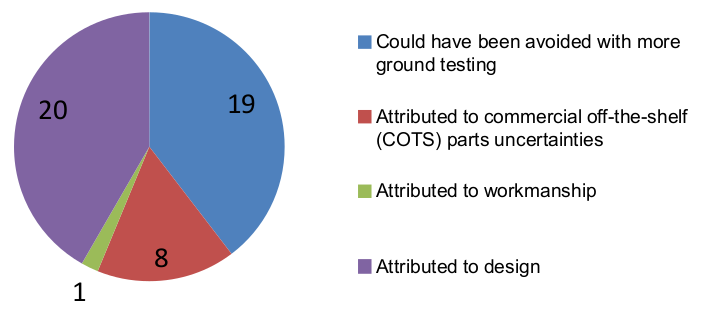
\includegraphics[height=4.5cm]{figure/cause_of_failure.png}
      \caption{故障原因に関する調査結果\cite{Venturini2017}}
      \label{fig:cause of failure}
\end{figure}

%ここへのつながり.別subsectionのほうがいいかも
%ほどよし信頼性工学のところをしっかりとまとめたほうがいい
また,大学衛星が商用利用や革新的なミッションに
挑戦するためには,超小型衛星のメリットである
コストの低さを十分に確保しながら,ほどほどの信頼性
を実現する「ほどよし」の考え方が
重要であると考えられている\cite{SHIRASAKA2011}.\\
故障に設計や製造の不良が含まれていることを考えると,
超小型衛星のほどほどの信頼性の評価を行うためには,
従来用いられてきた
各コンポーネントごとの信頼度の組み合わせでは不十分である.
そこで,設計・製造・運用における
信頼度を加味した評価手法が提案されている\cite{SHIRASAKA2011}.
式(\ref{eq:Reliability})が示すように,この評価手法では
設計や製造時の信頼性も重要な要素であると捉えられている.\\
超小型衛星のコストの低さを考慮すると,信頼性の高いコンポーネントを使用することによって
それぞれのコンポーネントの信頼性$R_{comp}$を高めるより,
設計や製造過程における信頼性を高めることが超小型衛星の信頼性の向上につながる.
また上述したように,超小型衛星の信頼性の低さの根本原因である設計不良や地上試験の不足
を改善していくことが,信頼性向上には不可欠である.

\begin{equation}
   R_{sat} = R_{des} \times R_{fab} \times R_{comp} \times R_{op} \label{eq:Reliability}
\end{equation}
\begin{table}[H]
   \centering
      \begin{tabular}{cl} 
        $R_{sat}$ & 衛星の真の信頼度\\
        $R_{des}$ & 設計における信頼度\\
        $R_{fab}$ & 製造における信頼度\\
        $R_{comp}$ & 衛星の信頼度(従来の信頼度)\\%コンポーネントの信頼度
        $R_{op}$ & 運用における信頼度
      \end{tabular}
\end{table}
%これを言うことで,この研究ではこれらのどこを高めているのかを考える必要がある.

%もうちょいちゃんと考える
\subsection{地上試験における問題}
以上で示したように,不具合の多くが設計,製造などに起因しているという問題がある.
一方で,これは超小型衛星開発のみに限られたことではなく,
中・大型衛星においても大きな問題となっている.
軌道上故障データを分析した結果\cite{SAITO2011}(図\ref{fig:error type})
によると,軌道上で
偶発的に発生した故障はわずか11%であり,それ以外は設計,製造などの開発
活動に起因するものであることが分かっている.\\
また,軌道上で発生した不具合が「地上試験で
発現しなかった,または発見できかった原因」が以下の
図\ref{fig:error cause}のように知られている.
試験設備の不足によって確認できなかったものや,故障発見までの
時間が長く地上試験で発見することが現実的で無いものに関しては,
コストとリソースの面から試験による対策では限界がある.
一方で,試験モードの不備や,地上試験で発現していたのにもかかわらず
発見できなかった不具合に関しては試験に対する習熟度が不足していること,
不具合・リスクの分析が不十分であることが推測される\cite{SAITO2011}.

\begin{figure}[H]
   \centering
      \begin{tabular}{c}
         \begin{minipage}{0.50\hsize}
         \centering
         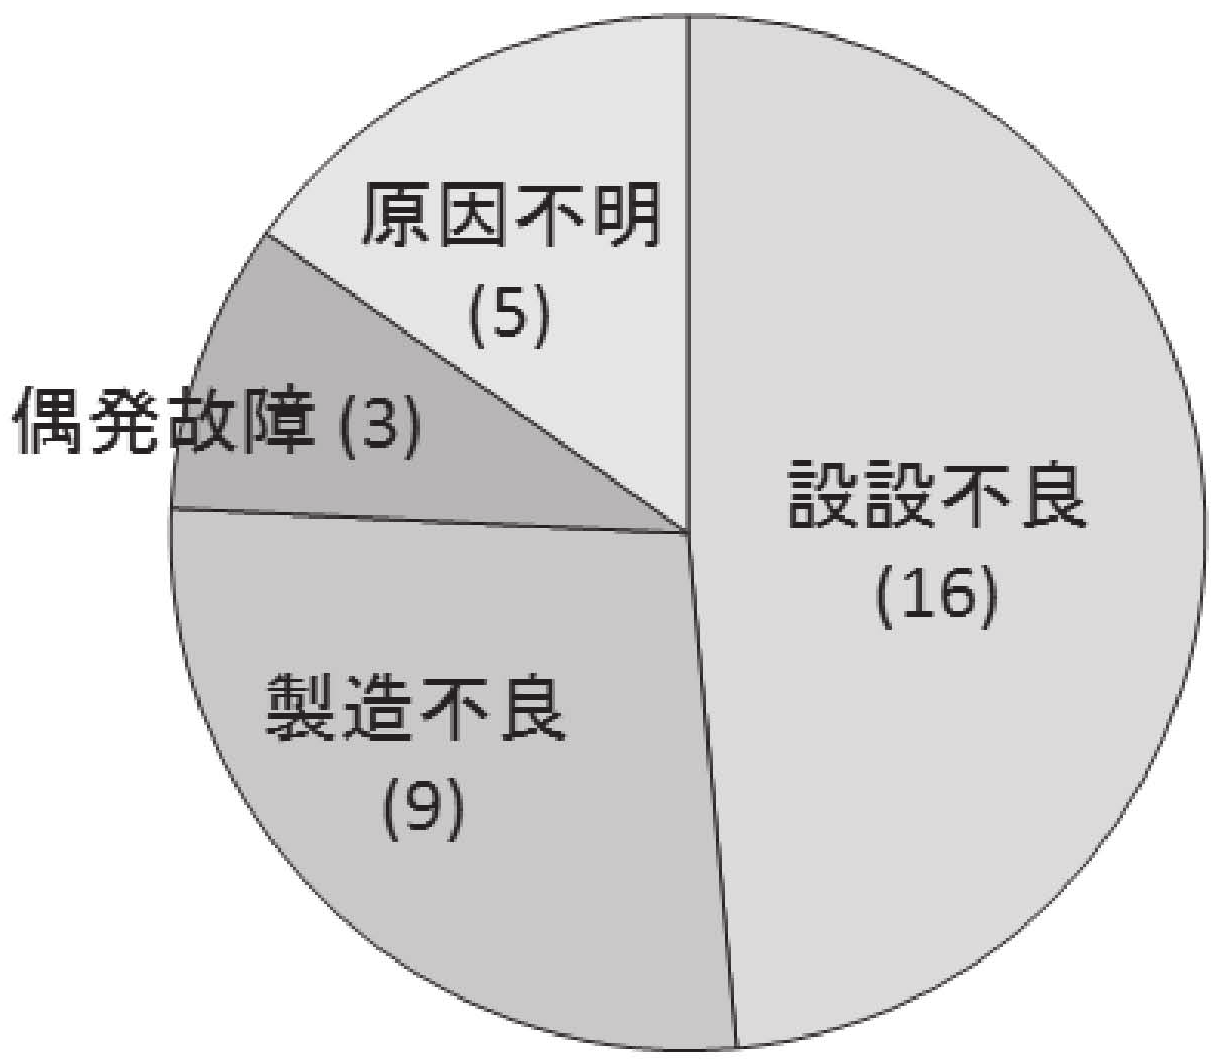
\includegraphics[width=5cm]{figure/on_orbit_error_tyoe.png}
            \caption{軌道上故障の原因類型の分布\cite{SAITO2011}}
            \label{fig:error type}
         \end{minipage}
         \begin{minipage}{0.50\hsize}
         \centering
         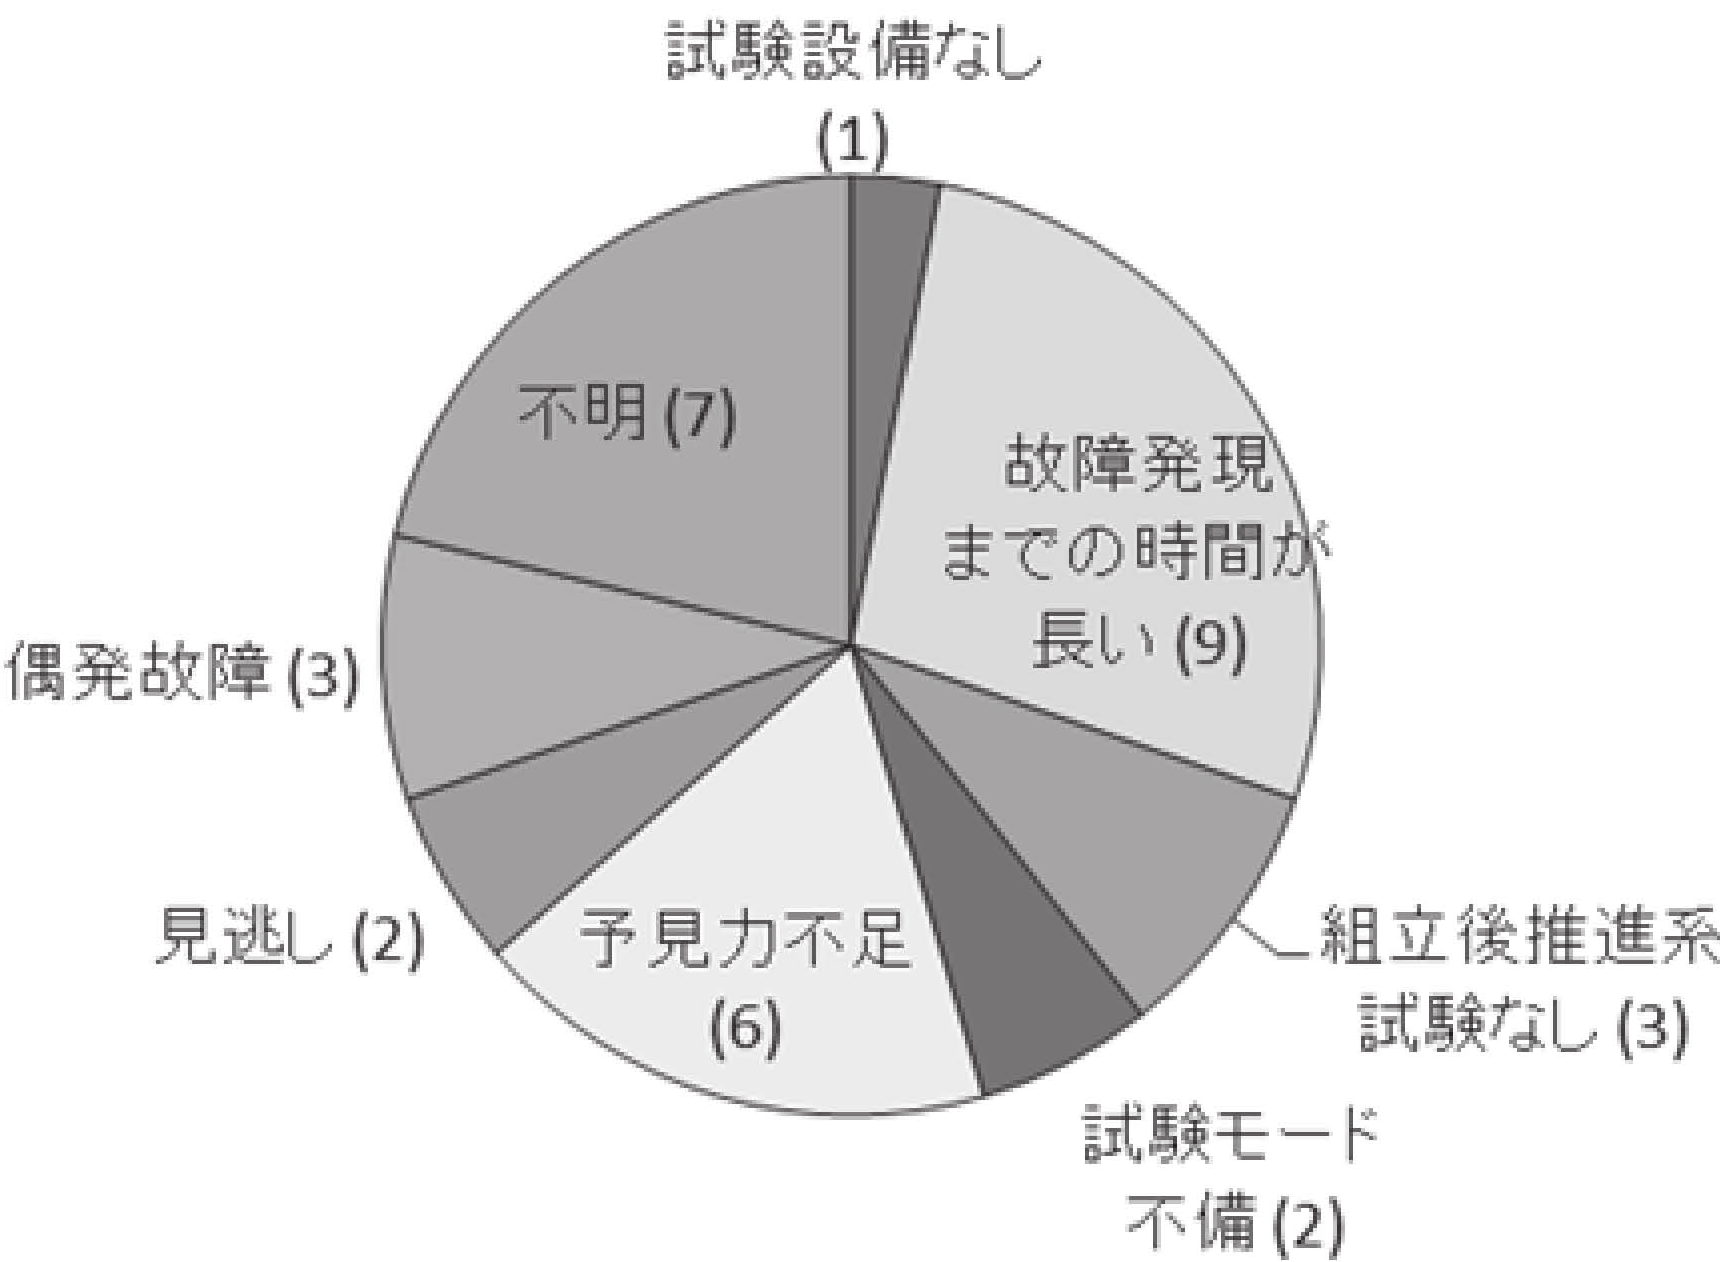
\includegraphics[height=5cm]{figure/not_found_error_seeds.png}
            \caption{軌道上故障の要因を地上で発見できなかった原因類型の分布\cite{SAITO2011}}
            \label{fig:error cause}
         \end{minipage}
      \end{tabular}  
\end{figure}

%ここに大学衛星の不具合分析に関する話があったような・・・・論文まとめから探し出せ

%ここの流れを見直す.根拠資料
\subsection{不具合原因特定の難しさ}
以上のように,衛星の不具合及びリスクの分析を,地上試験で十分に
行えていないことが,超小型衛星の信頼性の低さの原因の一つである.\\
そこで,地上試験で衛星の不具合及びリスク分析が十分に行えていない原因
を具体的に示すため,以下に人間による不具合分析の大まかな流れに関して一例を示す.
\begin{enumerate}[1)]
   \item 不具合が起きた際の衛星の状態を保存し記録に残す. 
   \item テレメトリから考えられる故障原因の候補を洗い出す.
   \item それらの故障の中でテレメトリから分かる情報を元に候補を棄却していく.
   \item 更に切り分けが必要な場合はコマンドを送り,
   それに対するテレメトリの挙動によって判断するという作業を繰り返す.
   \item 判断できない場合は,コンポーネントを取り出し直接確認を行う.
\end{enumerate}
まず,地上試験において十分に不具合分析が行えていない原因の1つとして,2)の故障原因の候補
の洗い出しを網羅的に行うことの難しさがある.\\
組み上げ状態の衛星から得られる情報は主にテレメトリのみである.
この際,衛星の内部状態を理解し,テレメトリから現在の衛星の状態
を類推することができなければ,十分に不具合原因の候補を洗い出すことは容易ではない.
また,衛星のように内部の機器が複雑に絡み合ったシステムでは,
人間が想定していない機器間のつながりが多数存在するため,不具合事象から全ての
故障可能性を洗い出すことは難しい.
本研究室の過去プロジェクト(PRISM)を対象にした研究では,
事前に人によって洗い出された故障モードは,%故障モードの意味
%ここの記述も微妙なので変更する
山口ら\cite{Yamaguchi2014}が構築したシステム
を用いて洗い出した故障モードと比較して,網羅性にかけていたという研究結果もある.
このように,人間による故障モードの洗い出しは思いつきによるものなので,
人の知識や経験に依存し,考えが及んでいないことで見逃している故障モードが多く存在する.

また,分析が不十分になっているもう一つの原因として,
3),4)の故障原因の切り分け作業の難しさがある.\\
上述したように超小型衛星は内部状態が複雑に絡み合っており,一つの不具合に対して
非常に多くの故障候補が洗い出される.
%切り分けを行うためのコマンドを探すのが難しい
そのため,多くの故障候補の中から切り分けを行い,最終的な故障を
特定するという作業は多くの知識と労力を必要とする作業である.
また,実ミッションで使用するコマンドとテレメトリは膨大な数であるため,
その中から切り分けを行うための情報を選択し,仮説の検証を行う作業は
無駄やヒューマンエラーを生むきっかけとなる.
不具合発生時は衛星の状態を十分に把握できていない状況であるため,
故障仮説を検証する際,未熟な運用者が不具合原因特定のために誤った%ここの表現改める
コマンドを送信してしまうと,意図しなかった動作を起こし
衛星の生存を脅かす危険性がある.
このため不具合原因特定を行う際には,不具合分析に用いるコマンドの安全性も
非常に重要な点である.

\subsection{不具合分析に関する先行研究}
上述のように,不具合原因の洗い出し
が網羅的にできていないこと,コマンドとテレメトリを用いて
原因特定を行う過程が知識依存になっていること
が,不具合分析が不十分になっている原因の一つであった.%一つでないが
これらの課題に対して,不具合分析に関する研究が盛んに行われている.
以下の表\ref{tab:previous_research}に,モデルに基づいて行う
機械などを対象にした不具合分析,故障診断手法に関してまとめた.
%比較軸が微妙過ぎる
\begin{table}[H]
   \centering
   \caption{不具合分析手法の比較}
   \label{tab:previous_research}
      \begin{tabular}{cccccc} \hline%もう少し示し方を考える.
         手法&故障網羅性&手法の目的%&モデル複雑度%専門家の知識が必要という点で?
         \\ \hline
         GDE&低&故障仮説生成%&低
         \\ %見てないし無くてもいいかも
         GDE+\cite{Struss1989}&中&故障仮説生成%&中
         \\
         網状故障解析\cite{Yamaguchi2014}&中&異常モード洗い出し%&高
         \\
         故障オントロジー\cite{Kitamura1999}&高&故障仮説生成%&高
         %\\
         %本手法&中%低かもしれない.接続関係しか見れていない
         %&故障箇所特定支援%もう少しよい表現がありそう.仮説検証支援
         %&中
         \\ \hline
      \end{tabular}
\end{table}
%モデル複雑度が比較の指標になるのか?
%モデルベースで行う不具合分析手法として一般的なものは
まず,GDEはモデルを元に行う不具合分析手法として一般的なもので
機器の正常時の制約モデルを元にして故障仮説の生成を行う.
GDEに対して,故障時モデルを組み込んだものがGDE+\cite{Struss1989}と呼ばれる手法であり,
入出力の観測結果から正常時との不整合を検知し,その不整合を説明するための仮説を洗い出す
ことを行っている.\\
%ここはそうなのか自身がない
%しかし,故障時モデルを組み込むためには事前に故障を洗い出す必要があり,
また,山口ら\cite{Yamaguchi2014}は,
衛星内部の機器の接続関係だけでなく,衛星が起こすアクションや状態などのつながりをモデル化し
想定していた機器間の接続関係からだけでは見えていなかった波及効果を洗い出すことを
可能にしている.\\
また,來村ら\cite{Kitamura1999}は故障を事象としてだけでなく,
時間経過や伝搬過程を含めて捉えるために必要となる概念を故障オントロジー\cite{Ontology1998}
として定義し,故障箇所に対する仮説だけでなく,より遡った故障原因に対する仮説を網羅的に生成する
手法を提案している.\\
\begin{comment}
   機器の正常時のモデルだけでなく,故障時モデルを組み込んだものや,
オントロジーを用いてプロセスのつながりまでモデル化したもの\cite{Yamaguchi2014},
異常伝播事象までモデル化して階層的な推論を行うもの\cite{Kitamura1999}などが
%不具合原因である機器の故障の原因などを探索可能にしたものなどが
あり,網羅的に故障候補を洗い出すために広く取り組まれている.
\end{comment}
以上のように故障仮説生成の研究に関しては,広く取り組まれている
一方で,來村ら\cite{Kitamura1999}が「効率の良い検証方法に関しては
今後の課題」と言及しているように,故障仮説の検証に取り組んだものは少ない.
%何か足りん気がする
上述したように,不具合分析は主に故障仮説の生成と故障仮説の検証作業から構成されるため,
検証過程に関しても取り組む必要性は十分にある.
また,故障候補の洗い出しを十分に行うことができたとしても,特定を行うことができなければ
地上試験によって設計や製造における不備を除くことができない.

\section{研究概要}
\subsection{本研究での目的}
以上を踏まえると,
不具合発生時に故障候補を洗い出し,その中から
原因を特定していく過程に,高い知識と経験が必要である
ことが,衛星の不具合やリスクの分析が不十分に
なっている原因の一つであると推察される.
また,故障候補の網羅的な洗い出し
に関しては広く取り組まれている一方で,仮説の検証作業の支援に関して
取り組んだ研究は十分に行われていない.

%機能に関しても箇条書きで分かりやすくできんか?
そこで本研究では,経験が浅く,衛星に関する知識の乏しいエンジニアであっても,
不具合事象から故障箇所の特定を行えるような以下の機能を満たす
不具合分析支援手法の提案を目的とする.
また,以下では不具合発生から故障箇所の特定を行う過程を「不具合分析」と表現している.\\

%これはどうするか要検討
\begin{itemize}
  \item 故障候補を確認するためのコマンド及びテレメトリを提案する.
  \item コマンドの選択肢を選ぶ際の判断の指標を定量的に提示する.
\end{itemize}
%ここに補足説明が必要かも?見直す

\subsection{本論文の構成}
本論文は次のような構成となっている.
第2章では,本研究で提案する不具合分析手法で
使用する衛星のモデル%衛星のモデルに関してはどこでもいい気がする.接続関係とかは必要
と不具合分析のアルゴリズム,探索された結果を選択する際に
必要となる指標に関して,コマンドの安全性と故障候補の切り分け能力の観点から述べている.
また,第3章では提案手法を実践した結果に関してまとめており,
本手法によって故障箇所特定のプロセスを体系化できたこと,
指標に関する考察を述べる.
また,第4章では本論文での結論として,まとめとして研究目的に対する
本研究の成果を述べ,今後の課題を示している.
%章番号と一致しているのかを確認する.

\expandafter\ifx\csname ifdraft\endcsname\relax
\end{document}
\fi